%% BioMed_Central_Tex_Template_v1.06
%%                                      %
%  bmc_article.tex            ver: 1.06 %
%                                       %

%%IMPORTANT: do not delete the first line of this template
%%It must be present to enable the BMC Submission system to
%%recognise this template!!

%%%%%%%%%%%%%%%%%%%%%%%%%%%%%%%%%%%%%%%%%
%%                                     %%
%%  LaTeX template for BioMed Central  %%
%%     journal article submissions     %%
%%                                     %%
%%          <8 June 2012>              %%
%%                                     %%
%%                                     %%
%%%%%%%%%%%%%%%%%%%%%%%%%%%%%%%%%%%%%%%%%


%%%%%%%%%%%%%%%%%%%%%%%%%%%%%%%%%%%%%%%%%%%%%%%%%%%%%%%%%%%%%%%%%%%%%
%%                                                                 %%
%% For instructions on how to fill out this Tex template           %%
%% document please refer to Readme.html and the instructions for   %%
%% authors page on the biomed central website                      %%
%% http://www.biomedcentral.com/info/authors/                      %%
%%                                                                 %%
%% Please do not use \input{...} to include other tex files.       %%
%% Submit your LaTeX manuscript as one .tex document.              %%
%%                                                                 %%
%% All additional figures and files should be attached             %%
%% separately and not embedded in the \TeX\ document itself.       %%
%%                                                                 %%
%% BioMed Central currently use the MikTex distribution of         %%
%% TeX for Windows) of TeX and LaTeX.  This is available from      %%
%% http://www.miktex.org                                           %%
%%                                                                 %%
%%%%%%%%%%%%%%%%%%%%%%%%%%%%%%%%%%%%%%%%%%%%%%%%%%%%%%%%%%%%%%%%%%%%%

%%% additional documentclass options:
%  [doublespacing]
%  [linenumbers]   - put the line numbers on margins

%%% loading packages, author definitions

%\documentclass[twocolumn]{bmcart}% uncomment this for twocolumn layout and comment line below
\documentclass{bmcart}

%%% Load packages
%\usepackage{amsthm,amsmath}
%\RequirePackage{natbib}
%\RequirePackage[authoryear]{natbib}% uncomment this for author-year bibliography
\RequirePackage{hyperref}
\usepackage[utf8]{inputenc} %unicode support
%\usepackage[applemac]{inputenc} %applemac support if unicode package fails
%\usepackage[latin1]{inputenc} %UNIX support if unicode package fails
\usepackage{graphicx}

\usepackage{cleveref}

\usepackage{biocon}
\newplant{At}{genus=Arabidopsis,epithet=thaliana}

%%%%%%%%%%%%%%%%%%%%%%%%%%%%%%%%%%%%%%%%%%%%%%%%%
%%                                             %%
%%  If you wish to display your graphics for   %%
%%  your own use using includegraphic or       %%
%%  includegraphics, then comment out the      %%
%%  following two lines of code.               %%
%%  NB: These line *must* be included when     %%
%%  submitting to BMC.                         %%
%%  All figure files must be submitted as      %%
%%  separate graphics through the BMC          %%
%%  submission process, not included in the    %%
%%  submitted article.                         %%
%%                                             %%
%%%%%%%%%%%%%%%%%%%%%%%%%%%%%%%%%%%%%%%%%%%%%%%%%


%\def\includegraphic{}
%\def\includegraphics{}



%%% Put your definitions there:
\startlocaldefs
\newcommand{\formatprogramnames}[1]{\texttt{#1}}
\newcommand{\ce}{\formatprogramnames{chloroExtractor}}
\newcommand{\oa}{\formatprogramnames{ORG.Asm}}
\newcommand{\fp}{\formatprogramnames{Fast-Plast}}
\newcommand{\ioga}{\formatprogramnames{IOGA}}
\newcommand{\np}{\formatprogramnames{NOVOPlasty}}
\newcommand{\go}{\formatprogramnames{GetOrganelle}}
\newcommand{\cassp}{\formatprogramnames{Chloroplast assembly protocol}}

% Niklas table
%\newcommand{\ok}{\textcolor[rgb]{0.7,0.7,0}{\textsc{\bfseries{}OKAY}}}
%\newcommand{\bad}{\textcolor{red}{\textsc{\bfseries{}BAD}}}
%\newcommand{\good}{\textcolor[rgb]{0,0.6,0}{\textsc{\bfseries{}GOOD}}}
\newcommand{\ok}{\textsc{Okay}}
\newcommand{\bad}{\textsc{Bad}}
\newcommand{\good}{\textsc{Good}}


% List of docker images
\newcommand{\docker}[2]{\href{https://cloud.docker.com/u/chloroextractorteam/repository/docker/chloroextractorteam/#1}{chloroextracteam/#1:#2}}
\newcommand{\dockerce}{\docker{benchmark\_chloroextractor}{v2.0.0}}
\newcommand{\dockercesha}{\texttt{8f49e03424b37e699c5fea9391f79dbb9f2d0dc550ce86c4c700f39deec2dacd}}
\newcommand{\dockeroa}{\docker{benchmark\_org-asm}{v2.0.0}}
\newcommand{\dockeroasha}{\texttt{ff83677c97b7c4e346191b9e04a5162eeea2a8dfd9e60ff84067d33747868f60}}
\newcommand{\dockerfp}{\docker{benchmark\_fastplast}{v2.0.0}}
\newcommand{\dockerfpsha}{\texttt{a3d06a610f8340ba49c3ff3b27342534e2a5348b17caa4fd3c3f3d327243a272}}
\newcommand{\dockerioga}{\docker{benchmark\_ioga}{v2.0.0}}
\newcommand{\dockeriogasha}{\texttt{4698a21c343c60290bbf16811165a654ff01e8fddeb41cd75d0771b7f45968c0}}
\newcommand{\dockernp}{\docker{benchmark\_novoplasty}{v2.0.0}}
\newcommand{\dockernpsha}{\texttt{106387bad4e8e5c53fb9d4c3bdd60cdddf05a47b52a38697369eeabb947c547c}}
\newcommand{\dockergo}{\docker{benchmark\_getorganelle}{v2.0.0}}
\newcommand{\dockergosha}{\texttt{2ed3a464a82025a196ea56c649d0b0a3472cef76994bb065d56054d93298d956}}
\newcommand{\dockercassp}{\docker{benchmark\_chloroplast\_assembly\_protocol}{v2.0.0}}
\newcommand{\dockercasspsha}{\texttt{d10d2317103d91fadec4cb1d5466ac109f23176ad74b6f44f0179175f050155d}}
\endlocaldefs


%%% Begin ...
\begin{document}

%%% Start of article front matter
\begin{frontmatter}

\begin{fmbox}
\dochead{Research}

%%%%%%%%%%%%%%%%%%%%%%%%%%%%%%%%%%%%%%%%%%%%%%
%%                                          %%
%% Enter the title of your article here     %%
%%                                          %%
%%%%%%%%%%%%%%%%%%%%%%%%%%%%%%%%%%%%%%%%%%%%%%

\title{The landscape of chloroplast genome assembly tools}

%%%%%%%%%%%%%%%%%%%%%%%%%%%%%%%%%%%%%%%%%%%%%%
%%                                          %%
%% Enter the authors here                   %%
%%                                          %%
%% Specify information, if available,       %%
%% in the form:                             %%
%%   <key>={<id1>,<id2>}                    %%
%%   <key>=                                 %%
%% Comment or delete the keys which are     %%
%% not used. Repeat \author command as much %%
%% as required.                             %%
%%                                          %%
%%%%%%%%%%%%%%%%%%%%%%%%%%%%%%%%%%%%%%%%%%%%%%

\author[
    addressref={aff2},
    noteref={n1},
    email={jan.freudenthal@uni-wuerzburg.de}
    ]{\inits{JAF}\fnm{Jan A} \snm{Freudenthal}}
\author[
    addressref={aff2},
    noteref={n1},
    email={simon-pfaff@gmx.de}
    ]{\inits{SP}\fnm{Simon} \snm{Pfaff}}
\author[
   addressref={aff2,aff3},
   email={niklas.terhoeven@uni-wuerzubrg.de}
]{\inits{NT}\fnm{Niklas} \snm{Terhoeven}}
\author[
   addressref={aff1,aff2},
   noteref={n2},
   email={markus.ankenbrand@uni-wuerzubrg.de}
]{\inits{MJA}\fnm{Markus J} \snm{Ankenbrand}}
\author[
   addressref={aff1,aff4},                   % id's of addresses, e.g. {aff1,aff2}
   corref={aff1},                       % id of corresponding address, if any
   noteref={n2},                        % id's of article notes, if any
   email={frank.foerster@uni-wuerzburg.de}   % email address
]{\inits{FF}\fnm{Frank} \snm{Förster}}


%%%%%%%%%%%%%%%%%%%%%%%%%%%%%%%%%%%%%%%%%%%%%%
%%                                          %%
%% Enter the authors' addresses here        %%
%%                                          %%
%% Repeat \address commands as much as      %%
%% required.                                %%
%%                                          %%
%%%%%%%%%%%%%%%%%%%%%%%%%%%%%%%%%%%%%%%%%%%%%%

\address[id=aff2]{%                           % unique id
  \orgname{Department of Bioinformatics, University of W\"{u}rzburg}, % university, etc
  \street{Biozentrum, Am Hubland},                     %
  \postcode{97074},                                % post or zip code
  \city{W\"{u}rzburg},                              % city
  \cny{Germany}                                    % country
}
\address[id=aff1]{%
  \orgname{Center for Computational and Theoretical Biology, University of W\"{u}rzburg},
  \street{Campus Hubland Nord},
  \postcode{97074}
  \city{W\"{u}rzburg},
  \cny{Germany}
}
\address[id=aff3]{%
  \orgname{AnaLife Data Science},
  \street{Friedrich-Bergius-Ring 15},
  \postcode{97076}
  \city{W\"{u}rzburg},
  \cny{Germany}
}
\address[id=aff4]{%
  \orgname{Fraunhofer IME-BR},
  \street{Winchester Str.\ 2},
  \postcode{97076}
  \city{Gie\ss{}en},
  \cny{Germany}
}

%%%%%%%%%%%%%%%%%%%%%%%%%%%%%%%%%%%%%%%%%%%%%%
%%                                          %%
%% Enter short notes here                   %%
%%                                          %%
%% Short notes will be after addresses      %%
%% on first page.                           %%
%%                                          %%
%%%%%%%%%%%%%%%%%%%%%%%%%%%%%%%%%%%%%%%%%%%%%%

\begin{artnotes}
%\note{Sample of title note}     % note to the article
\note[id=n1]{Equal contributor} % note, connected to author
\note[id=n2]{Corresponding author} % note, connected to author
\end{artnotes}

\end{fmbox}% comment this for two column layout

%%%%%%%%%%%%%%%%%%%%%%%%%%%%%%%%%%%%%%%%%%%%%%
%%                                          %%
%% The Abstract begins here                 %%
%%                                          %%
%% Please refer to the Instructions for     %%
%% authors on http://www.biomedcentral.com  %%
%% and include the section headings         %%
%% accordingly for your article type.       %%
%%                                          %%
%%%%%%%%%%%%%%%%%%%%%%%%%%%%%%%%%%%%%%%%%%%%%%

\begin{abstractbox}

\begin{abstract} % abstract
The special issue will accept manuscripts presenting:

- in-depth analyses of advantages

-limitations of state-of-the-art methods

-demonstration on a variety of representative datasets and simulations

-clear guidelines/recommendations for the end-user

-insight into future directions for methods
\parttitle{First part title} %if any
Text for this section.

\parttitle{Second part title} %if any
Text for this section.
\end{abstract}

%%%%%%%%%%%%%%%%%%%%%%%%%%%%%%%%%%%%%%%%%%%%%%
%%                                          %%
%% The keywords begin here                  %%
%%                                          %%
%% Put each keyword in separate \kwd{}.     %%
%%                                          %%
%%%%%%%%%%%%%%%%%%%%%%%%%%%%%%%%%%%%%%%%%%%%%%

\begin{keyword}
\kwd{Chloroplast}
\kwd{Genome assembly}
\kwd{author}
\end{keyword}

% MSC classifications codes, if any
%\begin{keyword}[class=AMS]
%\kwd[Primary ]{}
%\kwd{}
%\kwd[; secondary ]{}
%\end{keyword}

\end{abstractbox}
%
%\end{fmbox}% uncomment this for twcolumn layout

\end{frontmatter}

%%%%%%%%%%%%%%%%%%%%%%%%%%%%%%%%%%%%%%%%%%%%%%
%%                                          %%
%% The Main Body begins here                %%
%%                                          %%
%% Please refer to the instructions for     %%
%% authors on:                              %%
%% http://www.biomedcentral.com/info/authors%%
%% and include the section headings         %%
%% accordingly for your article type.       %%
%%                                          %%
%% See the Results and Discussion section   %%
%% for details on how to create sub-sections%%
%%                                          %%
%% use \cite{...} to cite references        %%
%%  \cite{koon} and                         %%
%%  \cite{oreg,khar,zvai,xjon,schn,pond}    %%
%%  \nocite{smith,marg,hunn,advi,koha,mouse}%%
%%                                          %%
%%%%%%%%%%%%%%%%%%%%%%%%%%%%%%%%%%%%%%%%%%%%%%

%%%%%%%%%%%%%%%%%%%%%%%%% start of article main body
% <put your article body there>

%%%%%%%%%%%%%%%%
%% Background %%
%%
\section*{Introduction}
\subsection*{General introduction and motivation}
Genome sequencing - important biological insights.
Eukaryotes have organelles with separate genomes.
Particularly, plants have chloroplasts beside mitochondria (generally chloroplast or plastid? plastid bit more general, I think also chromoplasts etc).
Chloroplast genome content and structure reviewed elsewhere \cite{wicke_evolution_2011,green_chloroplast_2011}.
Chloroplast genomes are widely used for evolutionary analyses.
Comparative genomics even more informative.
Complete chloroplast genome much easier to get than complete core genome.
But specific genome structure (esp. inverted repeat) makes automated resolution with short reads hard.
Many genome sequencing project contain chloroplast reads as a by-product even though that was not the aim of the study.
Resolved chloroplast helps to remove these reads which can improve assembly of the core.
Databases contain short read data for species where no reference chloroplast is available in the databases.
There is a lot of potential use cases for chloroplast genomes \cite{tonti-filippini_what_2017}
Resolving these would allow for more and larger scale comparative studies on whole chloroplasts.
Open question (?) structural variation across taxonomic groups.
Some researchers use shallow genome sequencing to reconstruct full chloroplast genomes for use as super-barcodes \cite{coissac_barcodes_2016}.

\subsection*{Chloroplast genome architecture}
Maybe separate section describing a prototypical chloroplast: LSC, IRa, SSC, IRb. Gene number and content. Size ranges. Evolutionary history incl. endosymbiontic gene transfer. Reduced genomes in parasitic plants. Loss of ndh gene family (maybe too specific). Preliminary SNP analysis in \plant{At} to estimate intraspecific variability? Is there anything known about intra-organismic variability (do some plants have multiple populations of chloroplasts? probably off topic).

\subsection*{Approaches to extracting chloroplasts from whole genome data}
1. Getting chloroplast reads out of mixed files
Mapping (potentially iterative), k-mer coverage analysis, seeded assembly
2. Assembly of chloroplast (incl special structure with IRs)
normal assembly - then blast, assembly then graph resolution, might be combined with step 1.

\subsection*{Purpose and scope of this study}
Clearly state criteria. Work with mixed data. Full automation. De novo - no manual selection of appropriate reference. No manual finishing. The step we are interested in is: from raw paired Illumina (!) reads to a fasta file containing the assembly (optimally full, circularized and on one contig). We are not interested in annotation or any additional contigs (genomic, mitochondrion, rRNA, etc.).
%\cite{koon,oreg,khar,zvai,xjon,schn,pond,smith,marg,hunn,advi,koha,mouse}

\section*{Methods}
Source code for all methods is available at \url{https://github.com/chloroExtractorTeam/benchmark} and archived under (zenodo doi).
All docker images are published on \url{https://cloud.docker.com/u/chloroextractorteam/} and are named with a leading \texttt{benchmark\_} (\cref{tab:dockerimages}).
datasets at (zenodo links for simulated and real).
This study adheres to the guidelines for computational method benchmarking \cite{weber_essential_2018}.

\subsection*{Inclusion Criteria}
List criteria that tools had to fulfill to be included in this study (maybe redundant with purpose and scope section).
List all programs that met the criteria with reference and very brief description:
\oa{}, \ce{}, \fp{}, \ioga{}, \np{}, \go{}, \cassp{}.
Name other relevant methods that were excluded (short description, reference, reason for exclusion).

\subsection*{Our Setup}
\dockerce{}

Defined interface, forward.fq and reverse.fq as only input. output.fa as only relevant output.
Docker container, all derived from main container, wrapper script makes all tools work conforming to the defined interface. Run docker containers for performance measurement and singularity containers on real datasets.
Singularity container were built from docker containers for usage on Julia-HPC of JMU using Singularity v.2.5.2 \cite{kurtzer2017singularity}
All singularity containers were run on the Julia-HPC on Intel® Xeon® Gold 6140 Processors using slurm workload manager version 17.11.8 \cite{Jette02slurm}. Assemblies run on 4 threads using 10 GB RAM with a timelimit of 48 hours 

\subsection*{Data}
\subsubsection*{Simulated}
\plant{At} (TAIR10). Perfect data, sliding window with seqkit (circular for chloro and mito). No errors, no insert size variation, perfect quality, equal coverage.

\subsubsection*{Real}
Datasets in SRA with reference chloroplast in cp database.
Total of 380 SRA samples selected (see supplementary table?).

\subsection*{Evaluation Criteria}
\subsubsection*{Computational Resources}
Description of our performance measurement with docker. List metrics that are monitored, I/O, CPU, memory, ...
On simulated dataset with different read counts and different number of threads given.

\subsubsection*{Qualitative}

The qualitative evaluation is mainly based on the reviewer guidelines for the Journal of Open Source Software (JOSS) \cite{joss}.
To create a standard environment, all tools were tested in a fresh default installation of Ubuntu 18.04.2 running in a virtual machine. The tools were installed according to their installation instructions and
the provided tutorial or example usage was executed. During the evaluation, the following
questions were asked:

\begin{itemize}
    \item Is the tool easy to install? 
    \item Is there a way to test the installation or a tutorial on how to use the tool? 
    \item Is there a good documentation on the parameter settings? 
    \item Is the tool maintained (issues answered, implementation of new features)? 
    \item Is the tool Open Source?
\end{itemize}

These questions were answered with \good{}, \ok{} or \bad{}, depending on the quality of the result. 
For example, a \good{} installation utilizes a automated package or dependency management like apt,
CRAN, docker, etc. An \ok{} installation procedure provides a custom script to install everything
or at least lists all dependencies. A \bad{} installation procedure fails to list important dependencies
or produces errors, that prevent a successful installation. 

After an initial evaluation, we contacted all authors via their github or gitlab issue tracking to
report any flaws we found.

\subsubsection*{Quantitative}
We want to quantify continuity, completeness, correctness, repeat resolution.
We use continuity: number of contigs.
Completeness: Number of covered bases on reference (when aligning assembly).
Correctness: Number of covered bases in assembly (when aligning reference).
Repeat resolution: Difference between above two measures (indicates collapsed or expanded repeats)
%
%\nocite{oreg,schn,pond,smith,marg,hunn,advi,koha,mouse}

Foreach dataset and assembler the proposed chloroplast was compared to the respective reference chloroplast using minimap2 v2.16 for pairwise alignment \cite{li2018minimap2}.

\[ score = 1 - \frac{1}{4} \cdot \left( |1- cov_{ref}| +  |1- cov_{qry}| + \left|1- e^{-\left| \ln{\frac{cov_{qry}}{cov_{ref}}}\right|}\right| + \left| 1 - \frac{1}{n_{contigs}} \right| \right) \]

Ich glaube diese Formel lässt sich vereinfachen zu:
\[ score = \frac{1}{4} \cdot \left( cov_{ref} +  cov_{qry} + e^{-\left| \ln{\frac{cov_{qry}}{cov_{ref}}}\right|} + \frac{1}{n_{contigs} }\right) \]


%% score = 1 - (abs(1-ref_cov_frac) + abs(1-qry_cov_frac) + abs(1-rep_res) + abs(1-(1/contig_num))))


\subsubsection*{reproducibility}
For reproducibility testing we randomly choose 100 data sets, that in the previous runs resulted in outputs for most of the assemblers and run them again with the same parameters as before. The resulting assemblies were scored again as described above and the scores of the 1. and the 2. run were compared to each other. 

\section*{Results}
\subsection*{Computational Resources}
Table and figure of performance evaluation. Including RAM, I/O, runtime, parallelization ability, CPU usage. Free text description of results, range, mean/median, effect of input size, threads parameter, ...

\subsection*{Qualitative}
Most of the tools were evaluated as mainly \good{} (see table \ref{tab:resultsQual}). However, a few critique points remained.
Two minor dependencies were missing in the \go{} installation instructions. There was also no test data available and an issue occurred when running it on a \plant{At} dataset. We are currently in the process of resolving this with the authors.

The \fp{} installation instructions were missing some dependencies. Like \go{}, \fp{} does not offer a test dataset or a tutorial, except from some example commands. 

The \oa{} installation instructions did not work. We found some issues, which are probably related to the requirement of python3.7. There is a tutorial with sample data available. However following the instructions resulted in a segmentation fault. We found a workaround for this bug and contacted the authors.

The main critique point of \np{} was the lack of a test dataset with instructions. This was fixed by the authors after we contacted them. \np{} uses a custom license. An OSI approved license would be preferred here.

The \ce{} does come with a test dataset and a short tutorial. However, a way to evaluate the results of the test run would be nice.

The \ioga{} installation instructions were missing many dependencies. Also, there was no test data or tutorial available and there is no license assigned to it. Since there was no update to the github repository for the last three years, the project can be seen as inactive. After contact, the authors promised to resolve the mentioned issues.

As many of the other tools, the installation instructions for the \cassp{} were missing some dependencies. The list was updated after we contacted the authors. This tool does come with a test dataset, however a note about the expected outcome would be nice. A more extensive tutorial is provided. The description about the parameter is short, but seems to be sufficient.

\subsection*{Quantitative}
\subsubsection*{Simulated data}
\textit{tile plot for simulated data goes here}
The only assembler obtaining perfect results according to our score for the simulated datasets is \go{}.
\ioga{} and \cassp{} showed the worst performance being unable to fully assemble a single chloroplast out of 14.
\np{} performed second best with scores above 80 for all datasets, only failing to resolve the chloroplast contig into one single circular assembly.
(As could have been expected -> discussion) the overall performance is best, when the input data consists purely of chloroplast reads.
Only \ioga{} and \cassp{} failed to deliver any results once each.
Besides that no clear causality between length of the input reads, ratio of core vs chloroplast reads and the performance can be clearly observed. 

\subsubsection*{real data sets}
Highest scoring is \go{} next is \fp{} while \ioga{} and \cassp{} perform poorly, never reaching a score of 1 (figure 1). TODO: median/mean score, mad/sd Tabelle

\textit{swarm plot goes here}
%% Den upset plot eventuell erst in die Discussion reinbringen ? Da wir davon ableiten welche tools wir empfehlen?


\subsubsection{Reproducability}
\textit{plot repro.pdf goes here}


\subsection*{Performance metrics}

\subsubsection*{Time requirements}

\textit{plot comp\_time\_log.pdf goes here}


\subsubsection*{Memory and CPU Usage }
\textit{plot usage\_amout\_threads.pdf goes here}


\[ CAP_n=221 , CE_n=205 , Fast-Plast_n=352 , GetOrganelle_n=356 IOGA_n=296, NOVOPlasty_n=270 org.ASM_n=228 \]




\section*{Discussion}
Discuss Computational Resources. Implications of very long running. Also state minimum requirements on the hardware (RAM, CPUs, storage). Importance of this depends on use case (if goal is one single chloroplast 

We evaluated all tools under the assumption that they are used in the most basic form (default parameters, no hand selected reference, no pre-processing of the data or post-processing of the result, restricted runtime). It is important to note that any tool might perform significantly different if parameters and references are fine-tuned for each dataset.

\subsection*{Clear guidelines for the end-user}
Which program (or combination of programs) to use? Does the decision depend on some parameter of the data (read length, amount, taxonomic group, ...)?

\subsection*{Ideas for future development}
Combining components from different tools might be a promising approach. E.g. read scaling from \ce{}, assembly from \go{} and structural resolution with fast-plast.
Mitigate installation issues e.g. by containerization.
Improve documentation and usability.
Maybe better integrated guessing of parameters (?) at least for automatization (but also because users tend to run a tool with default settings and look on what they get, only powerusers tweak parameters - and if it is possible to get a full chloroplast by guessing the best parameters there is no need for specific knowledge of parameters and their effects by the end user).
Other (more) data types, PacBio, nanopore.

\section*{Conclusion}
Short summary of clear guidelines and future development (might not be necessary as these are the last two sections of the Discussion anyway, so we might elect to skip this).

Put results back in context: the multitude of available tools shows importance to solve the challenge of chloro extraction. Presented benchmarking shows that all tools sometimes struggle even with ``perfect'' data. Although no program works everytime, most chloroplasts are resolved by at least one tool (is that so?). So programs are complementary, more effort to combine strengths of different methods (or automatic parameter selection - if failure is due to suboptimal parameters for the specific dataset).

Outlook: next step in the pipeline is annotation. There is a similar problem: many tools, which one to use? 
A large scale study reconstructing chloroplasts throughout SRA (or 1001 genome project) is feasible and promising using the existing tools (estimated runtime, number of novel chloroplasts).

%%%%%%%%%%%%%%%%%%%%%%%%%%%%%%%%%%%%%%%%%%%%%%
%%                                          %%
%% Backmatter begins here                   %%
%%                                          %%
%%%%%%%%%%%%%%%%%%%%%%%%%%%%%%%%%%%%%%%%%%%%%%

\begin{backmatter}

\section*{Competing interests}
  The authors disclose that SP, NT, FF, and MJA are developers of \ce{}, one of the tools benchmarked in this article. The authors exercised caution not to let this fact unfairly influence their judgement.

\section*{Author's contributions}
    MJA and FF conceived of the presented idea and supervised the findings of this manuscript.
SP and FF created the docker images.
NT performed the qualitative analysis for all assemblers.
MJA prepared the simulated and real data sets.
JAF assembled the real data sets.
FF ran the performance assemblies on the simulated data sets.
All authors developed the score model.
JAF and MJA implemented the score model and prepared the figures.
All authors discussed the results and contributed to the final manuscript.

\section*{Acknowledgements}
  Text for this section \ldots
%%%%%%%%%%%%%%%%%%%%%%%%%%%%%%%%%%%%%%%%%%%%%%%%%%%%%%%%%%%%%
%%                  The Bibliography                       %%
%%                                                         %%
%%  Bmc_mathpys.bst  will be used to                       %%
%%  create a .BBL file for submission.                     %%
%%  After submission of the .TEX file,                     %%
%%  you will be prompted to submit your .BBL file.         %%
%%                                                         %%
%%                                                         %%
%%  Note that the displayed Bibliography will not          %%
%%  necessarily be rendered by Latex exactly as specified  %%
%%  in the online Instructions for Authors.                %%
%%                                                         %%
%%%%%%%%%%%%%%%%%%%%%%%%%%%%%%%%%%%%%%%%%%%%%%%%%%%%%%%%%%%%%

% if your bibliography is in bibtex format, use those commands:
\bibliographystyle{bmc-mathphys} % Style BST file (bmc-mathphys, vancouver, spbasic).
\bibliography{bmc_article}      % Bibliography file (usually '*.bib' )
% for author-year bibliography (bmc-mathphys or spbasic)
% a) write to bib file (bmc-mathphys only)
% @settings{label, options="nameyear"}
% b) uncomment next line
%\nocite{label}

% or include bibliography directly:
% \begin{thebibliography}
% \bibitem{b1}
% \end{thebibliography}

%%%%%%%%%%%%%%%%%%%%%%%%%%%%%%%%%%%
%%                               %%
%% Figures                       %%
%%                               %%
%% NB: this is for captions and  %%
%% Titles. All graphics must be  %%
%% submitted separately and NOT  %%
%% included in the Tex document  %%
%%                               %%
%%%%%%%%%%%%%%%%%%%%%%%%%%%%%%%%%%%

%%
%% Do not use \listoffigures as most will included as separate files

\section*{Figures}
  \begin{figure}[h!]
  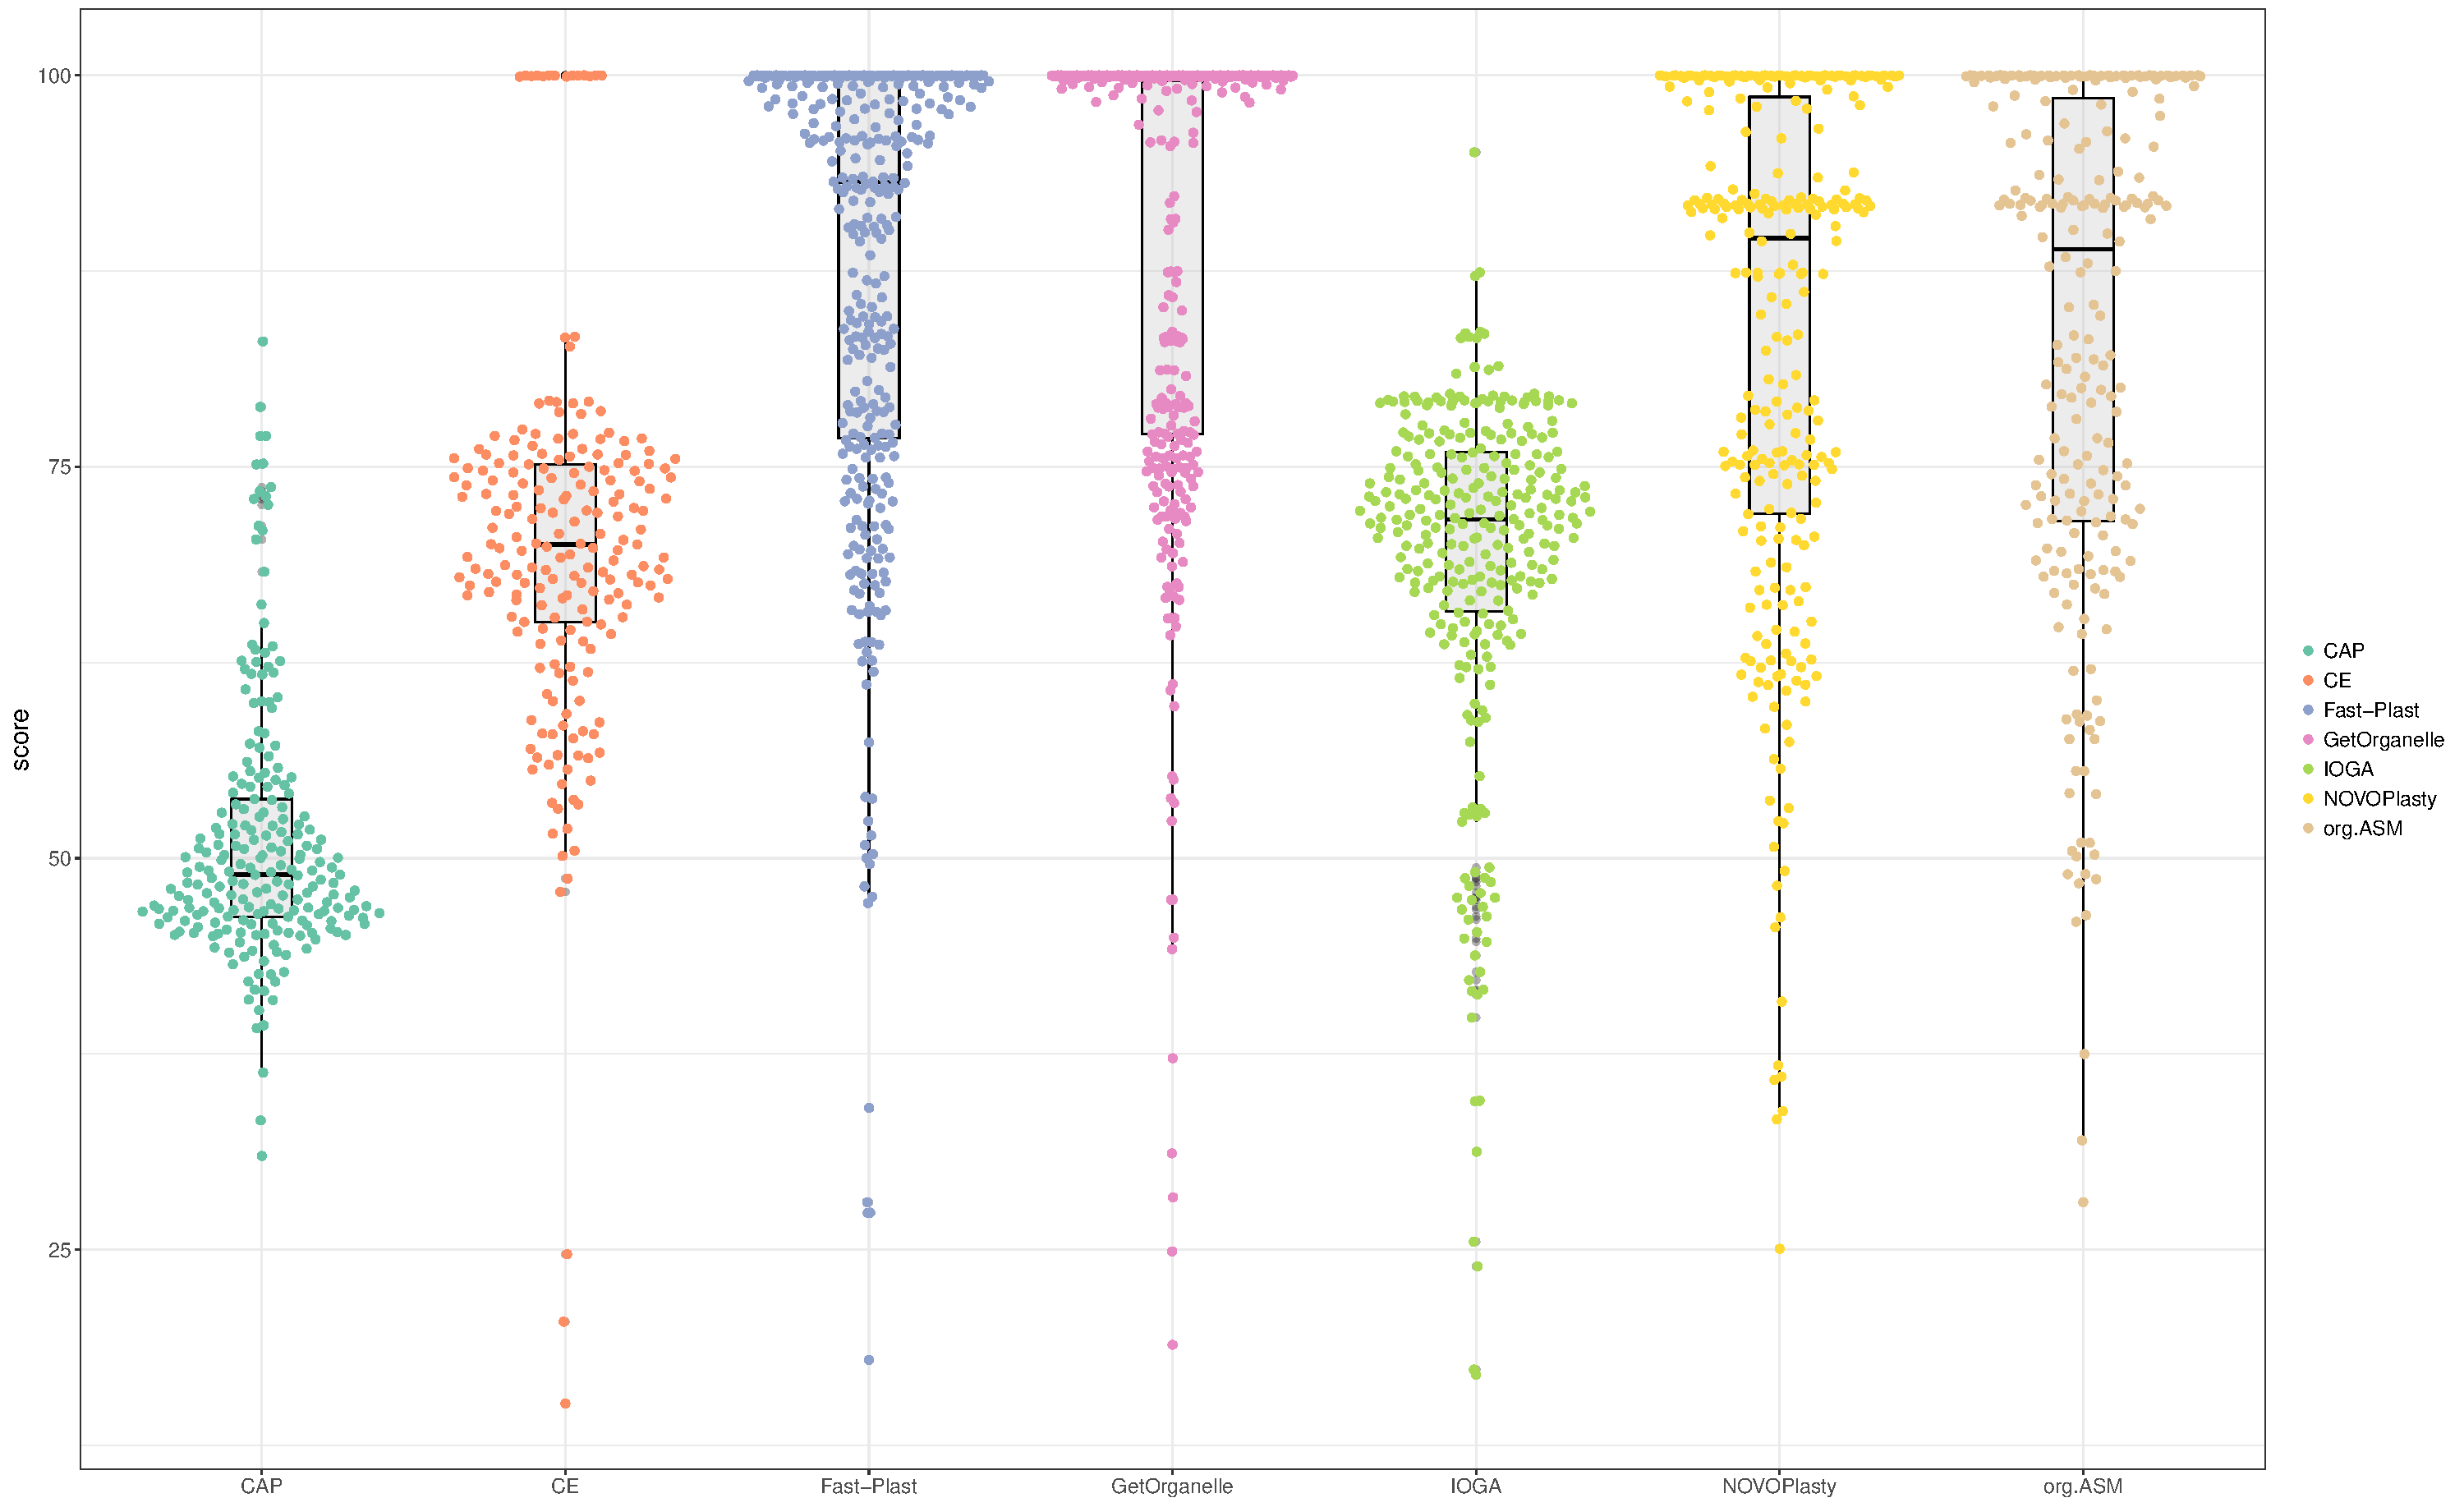
\includegraphics[width=\textwidth]{plots/swarm.pdf}
  \caption{\csentence{Sample figure title.}
      A short description of the figure content
      should go here.}
      \end{figure}

\begin{figure}[h!]
  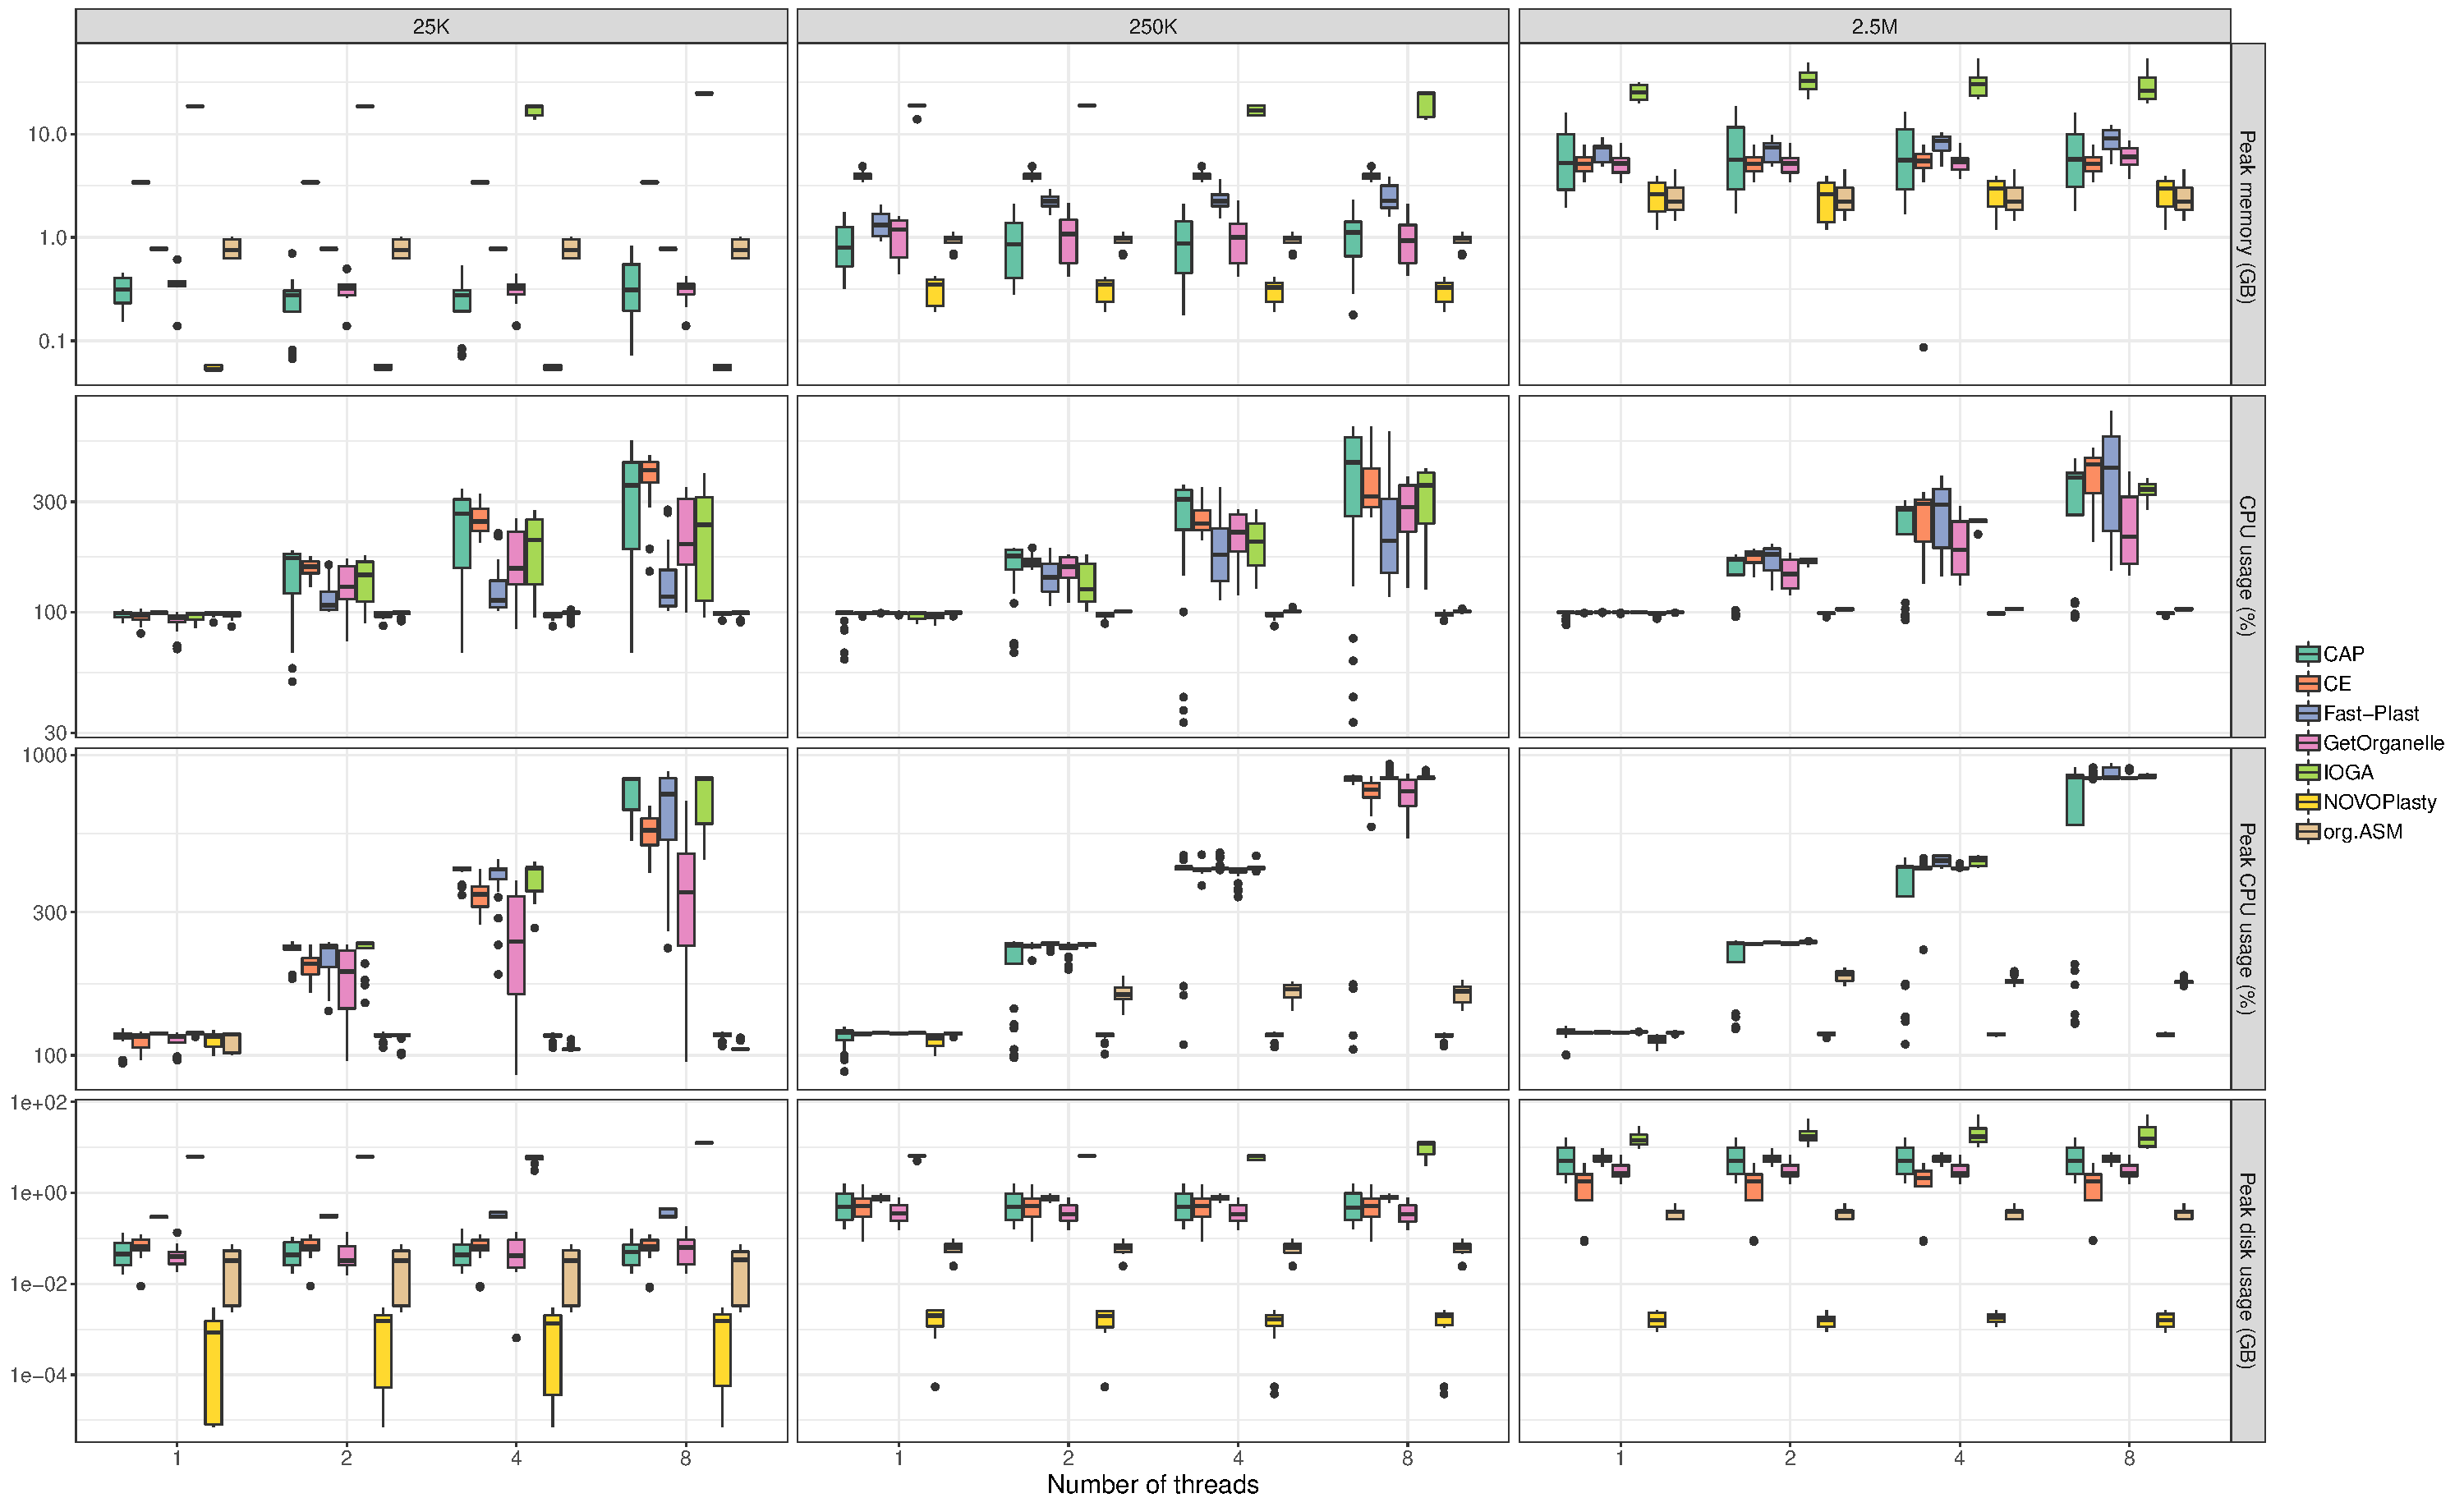
\includegraphics[width=\textwidth]{plots/usage_amount_threads.pdf}
  \caption{\csentence{Sample figure title.}
      Figure legend text.}
      \end{figure}

\begin{figure}[h!]
  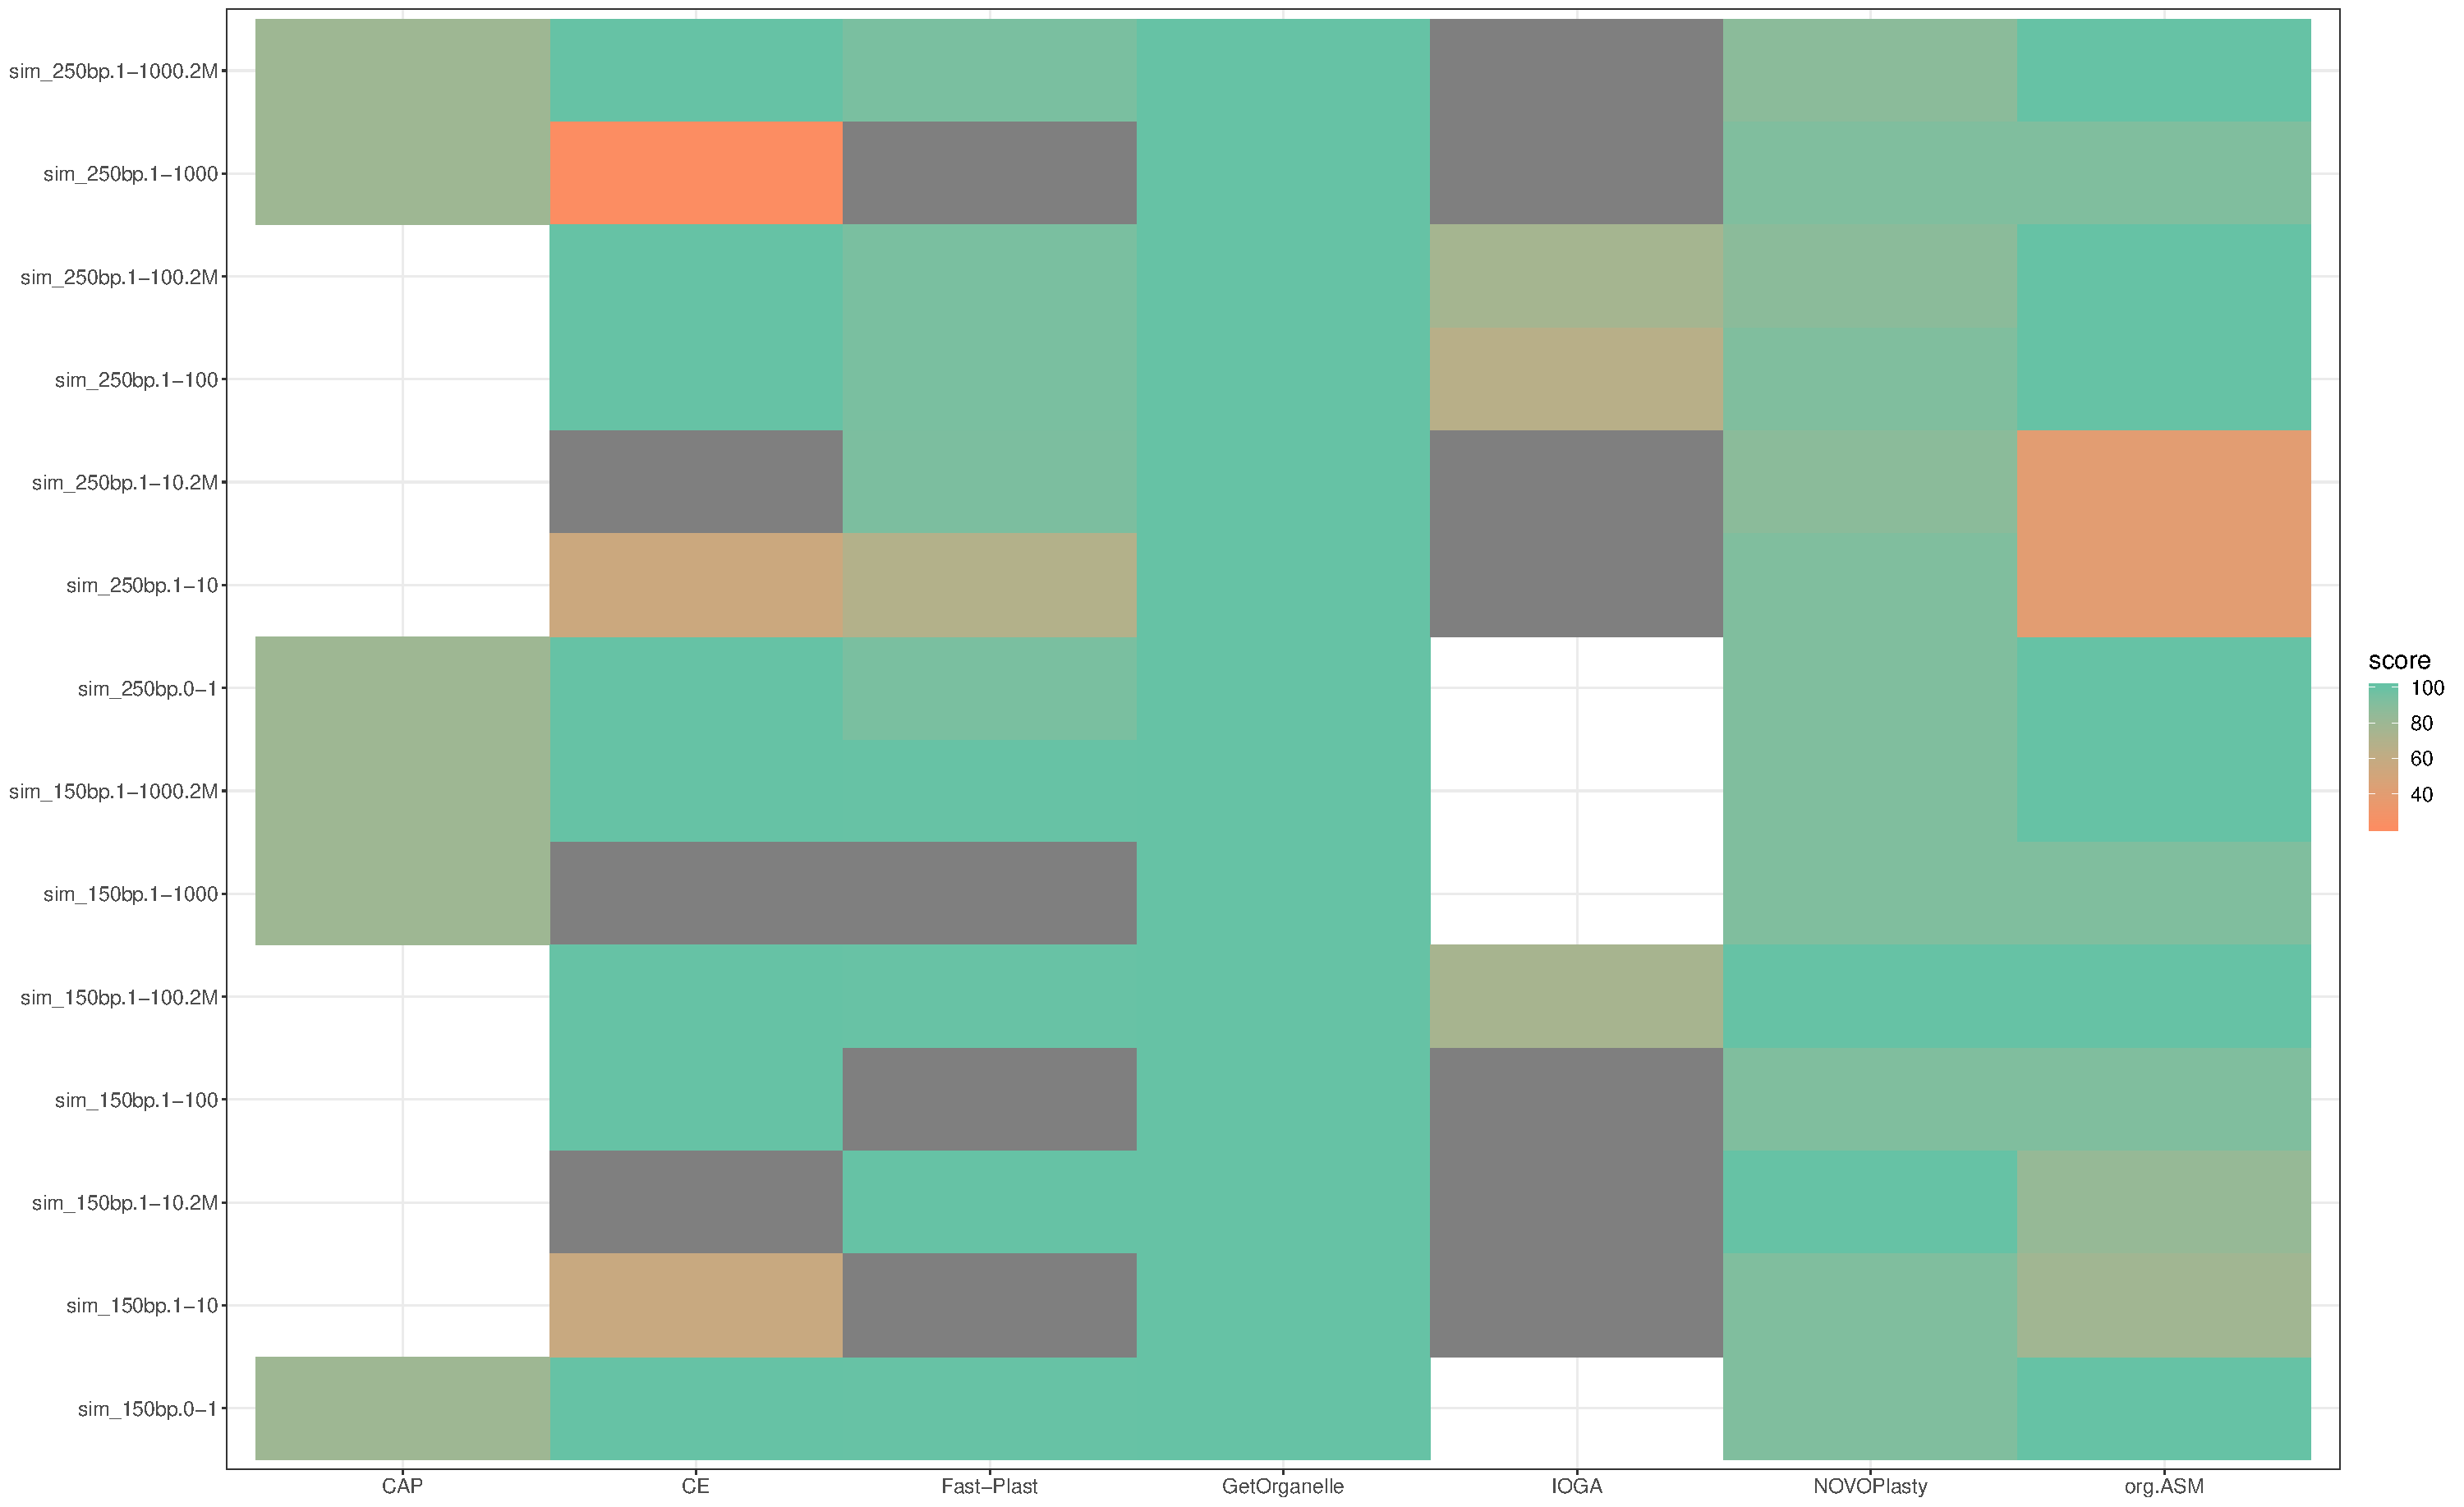
\includegraphics[width=\textwidth]{plots/sim_tiles.pdf}
  \caption{\csentence{Sample figure title.}
      Figure legend text.}
      \end{figure}

\begin{figure}[h!]
  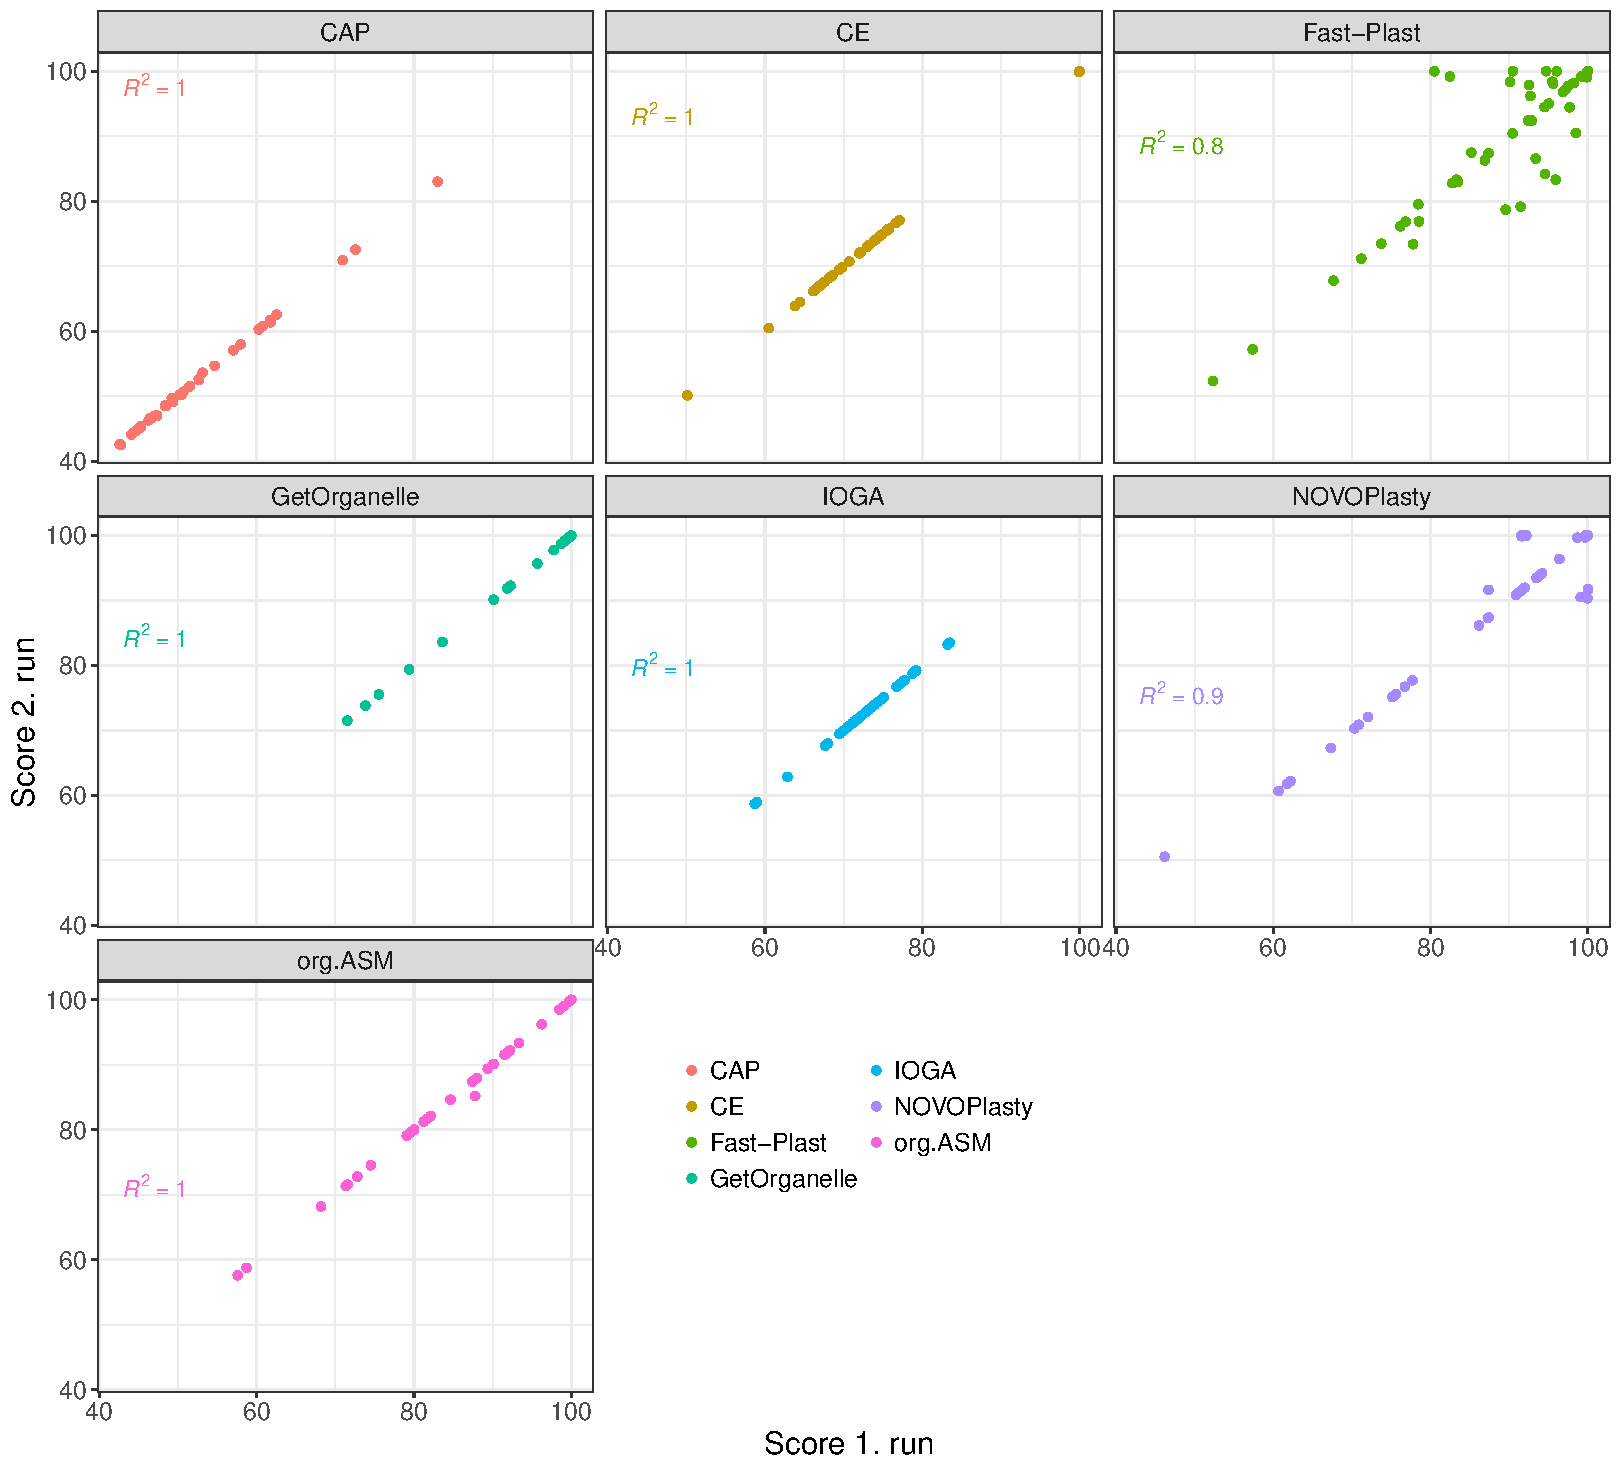
\includegraphics[width=\textwidth]{plots/repro.pdf}
  \caption{\csentence{Sample figure title.}
      Figure legend text.}
      \end{figure}

\begin{figure}[h!]
  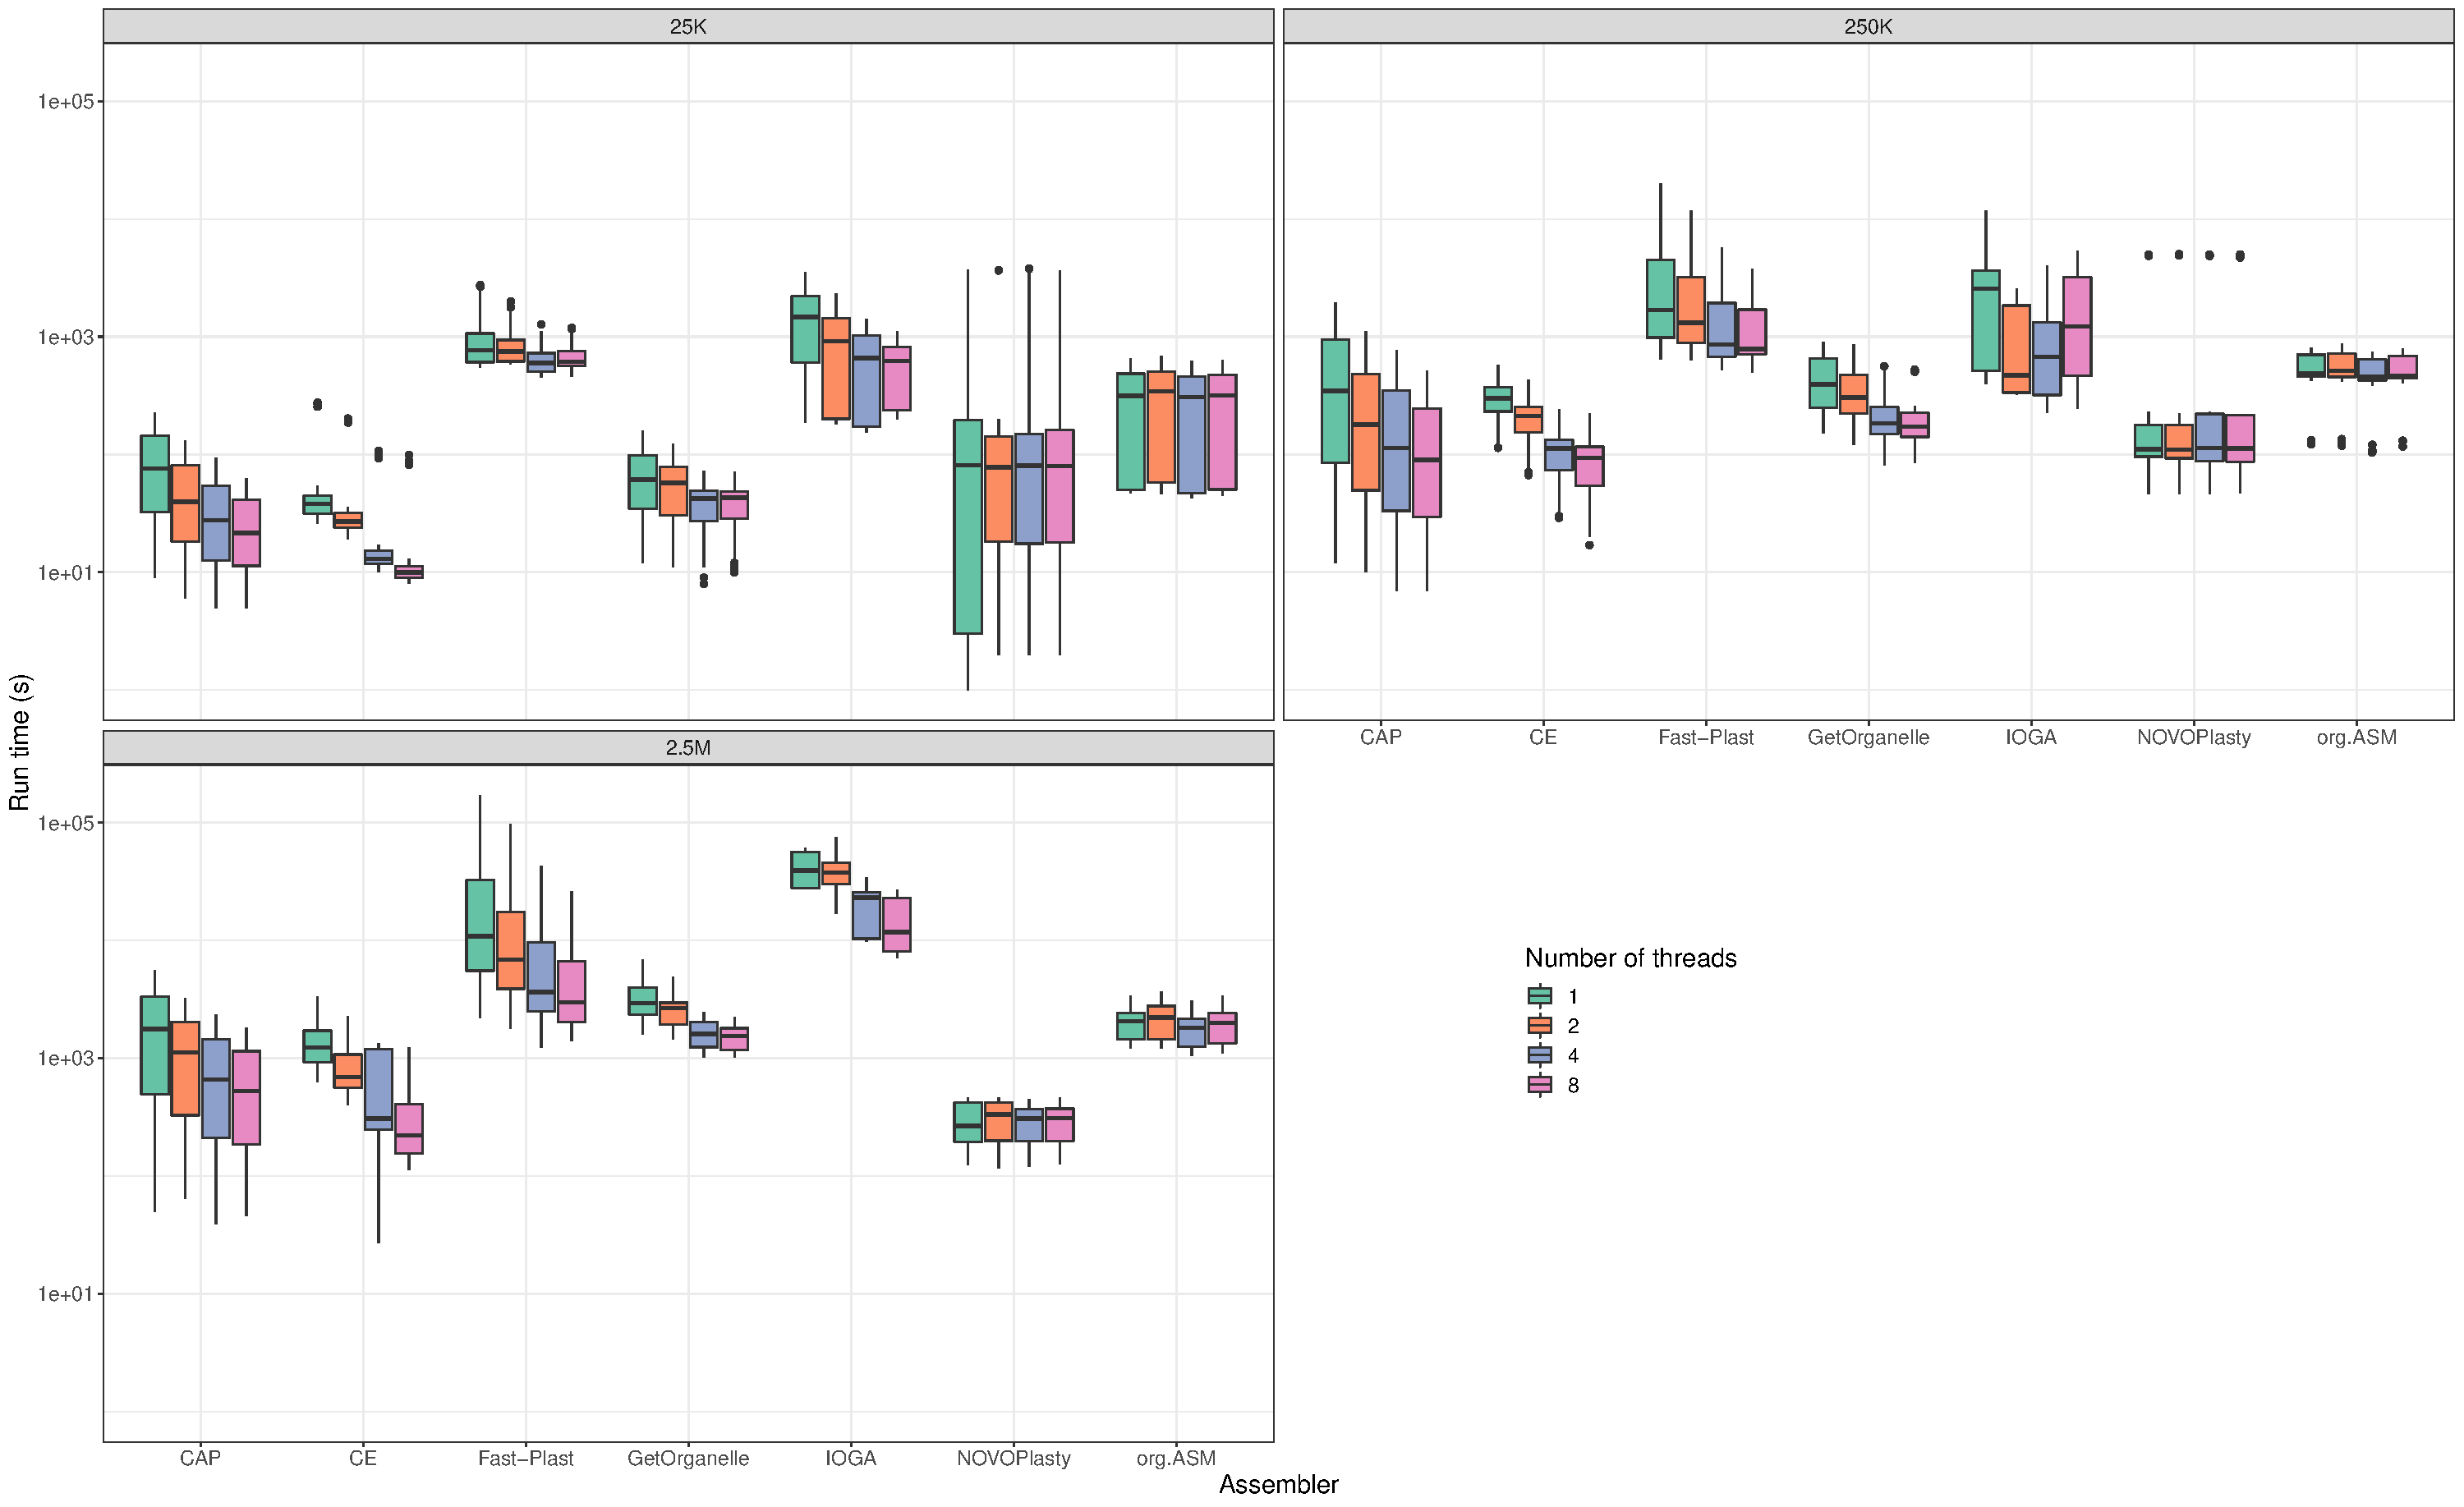
\includegraphics[width=\textwidth]{plots/comp_time_log.pdf}
  \caption{\csentence{Sample figure title.}
      Figure legend text.}
      \end{figure}

\begin{figure}[h!]
  
\includegraphics[width=\textwidth,page=2]{plots/upset.pdf}
  \caption{\csentence{Sample figure title.}
      Figure legend text.}
      \end{figure}

\begin{figure}[h!]
  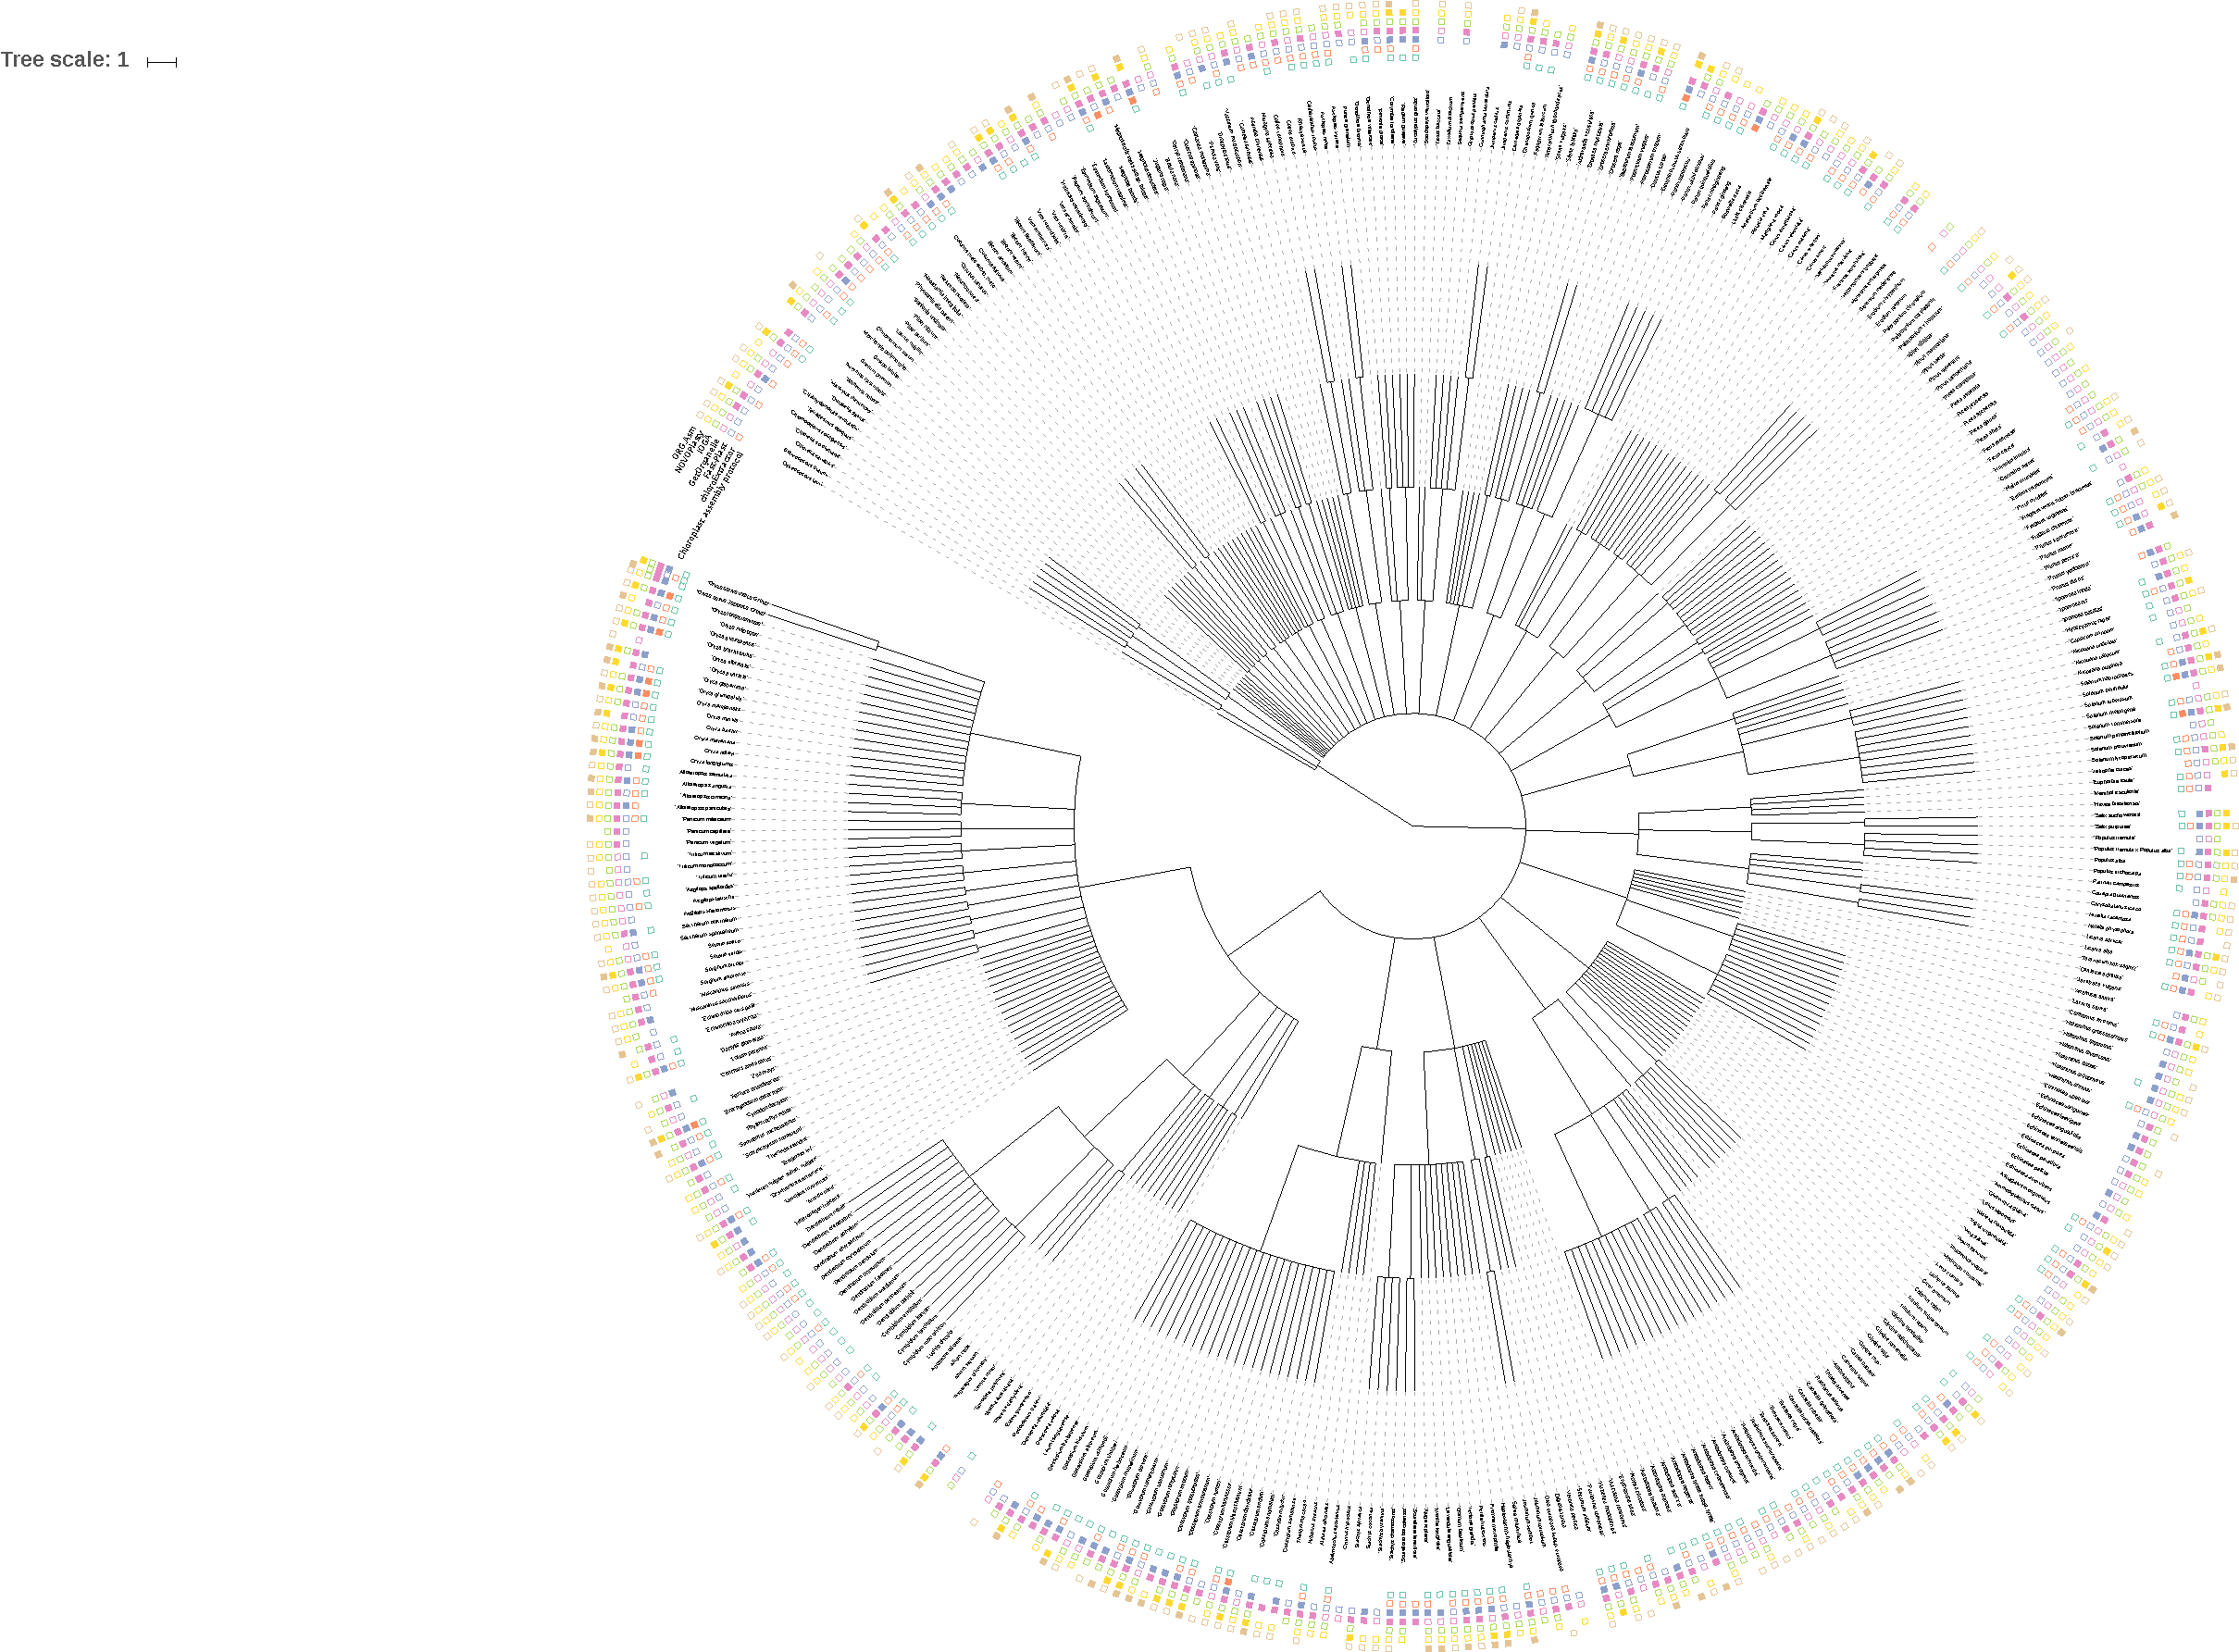
\includegraphics[width=\textwidth]{plots/real_datasets_tree.pdf}
  \caption{\csentence{Sample figure title.}
      Figure legend text.}
      \end{figure}

%%%%%%%%%%%%%%%%%%%%%%%%%%%%%%%%%%%
%%                               %%
%% Tables                        %%
%%                               %%
%%%%%%%%%%%%%%%%%%%%%%%%%%%%%%%%%%%

%% Use of \listoftables is discouraged.
%%
\section*{Tables}
\begin{table}[]
    \centering
    \caption{Overview of the results of the qualitative usability evaluation. Each tool 
    could score \good{}, \ok{} or \bad{} in each of the categories.}
    \label{tab:resultsQual}
\begin{tabular}{p{3cm}cccccc}   
Tool & Installation & Test/Tutorial & Documentation & Maintenance & FLOSS\\                           \hline \ce{}     &  \good{}  &  \good{}  &  \good{}  &  \good{}  &  \good{} \\
\cassp{}  &  \ok{}    &  \good{}  &  \ok{}    &  \good{}  &  \good{} \\
\fp{}     &  \bad{}   &  \ok{}    &  \good{}  &  \good{}  &  \good{} \\
\go{}     &  \ok{}    &  \ok{}    &  \good{}  &  \good{}  &  \good{} \\
\ioga{}   &  \bad{}   &  \bad{}   &  \ok{}    &  \ok{}    &  \bad{}  \\
\np{}     &  \good{}  &  \good{}  &  \good{}  &  \good{}  &  \ok{}   \\
\oa{}     &  \bad{}   &  \bad{}   &  \ok{}    &  \good{}  &  \good{} \\ \hline
\end{tabular}      
\end{table}

\begin{table}[h!]
\caption{Docker images used in our benchmark setup.}
\label{tab:dockerimages}
\centering
      \resizebox{\textwidth}{!}{\begin{tabular}{ccc}
        \hline
          Tool & Image name and tag & SHA256 Checksum   \\ \hline
          \ce & \dockerce & \dockercesha \\
          \cassp & \dockercassp & \dockercasspsha \\
          \fp & \dockerfp & \dockerfpsha \\
          \go & \dockergo & \dockergosha \\
          \ioga & \dockerioga & \dockeriogasha \\
          \np & \dockernp & \dockernpsha \\
          \oa & \dockeroa & \dockeroasha \\ \hline
      \end{tabular}}
\end{table}

\begin{table}[h!]
\caption{Sample table title. This is where the description of the table should go.}
      \begin{tabular}{cccc}
        \hline
           & B1  &B2   & B3\\ \hline
        A1 & 0.1 & 0.2 & 0.3\\
        A2 & ... & ..  & .\\
        A3 & ..  & .   & .\\ \hline
      \end{tabular}
\end{table}

%%%%%%%%%%%%%%%%%%%%%%%%%%%%%%%%%%%
%%                               %%
%% Additional Files              %%
%%                               %%
%%%%%%%%%%%%%%%%%%%%%%%%%%%%%%%%%%%

\section*{Additional Files}
  \subsection*{Additional file 1 --- Sample additional file title}
    Additional file descriptions text (including details of how to
    view the file, if it is in a non-standard format or the file extension).  This might
    refer to a multi-page table or a figure.

  \subsection*{Additional file 2 --- Sample additional file title}
    Additional file descriptions text.


\end{backmatter}
\end{document}
